\newpage
\section{Implementation}
The hardware description of the implemented game pong is divided into six modules. Firstly the video controller, which implements the VGA respectively HDMI interface, provides the functionality to display the video output on a monitor. Two modules generate the inputs for the movement of the paddles. The right paddle is controlled by the debounced up and down buttons of the board and the right paddle is controlled by the computer opponent. Additionally the image generator creates all required objects like the ball and paddles as well as their movement. Furthermore the match controller manages the interactions between the objects and the state of the match itself. Lastly the audio output is created by the sound generator module.
	\subsection{Video Controller}
    The video controller provides an interface for the image generator so objects can easily be displayed on a monitor. Thereby it makes the coordinates of the current pixel available and hides all additional requirements of the protocol like timing. The point of origin of the pixel matrix is located at the top left corner of the monitor. Because our group has access to the Atlys Spartan-6 board with HDMI connector as well as the Nexys 4 board with VGA connector, we decided to implement a video controller for both protocols, so the remaining modules could be implemented using both boards. The main focus was laid on the above mentioned uniform interface for the image generator so the remaining development is independent of the used video controller.
        \subsubsection{VGA Controller}
        \subsubsection{HDMI Controller}
    \subsection{Debouncer}
    \subsection{Computer Opponent}
    \subsection{Image Generator}
	\begin{figure}[here]
		\centering
		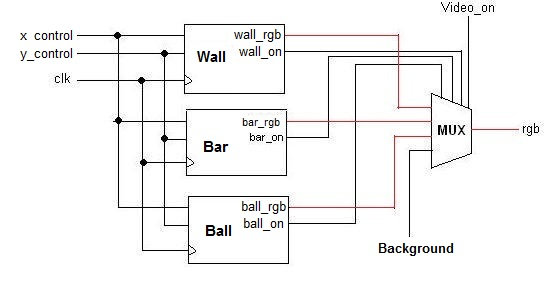
\includegraphics[scale=0.7]{images/img_gen.jpg}
		\caption{Schematic of the Image Generator}
		\label{img_gen}
	\end{figure}
        The Image Generator takes inputs from the players and outputs the video that can be displayed through the HDMI interface of the Atlys board. The panels shown in figure \ref{ball_wall_panel} are submodules of the module \texttt{image\_generator\_c}.
		This module calculates the movement of the ball and movement the two panels that are controlled by the players. 
		
		The movement of the ball is done by the \texttt{ball\_c} module. (see next Section for more details on implementation).
		After a well determined time frame, the ball's movement direction is determined and the next \texttt{x\_pos} and \texttt{y\_pos} are either incremented or decremented. 
		
		The module \texttt{panel\_c} determines the y-coordinate of on panel based on the player input. For instance, pressing \texttt{btn\_up} increments the \texttt{y\_pos} signal if the panel did not reach the top edge already. 


    \subsection{Match Controller}
    \subsection{Sound Generator}
        In order to generate sound, we used the on board LM4550 chip
	\begin{figure}[here]
		\centering
		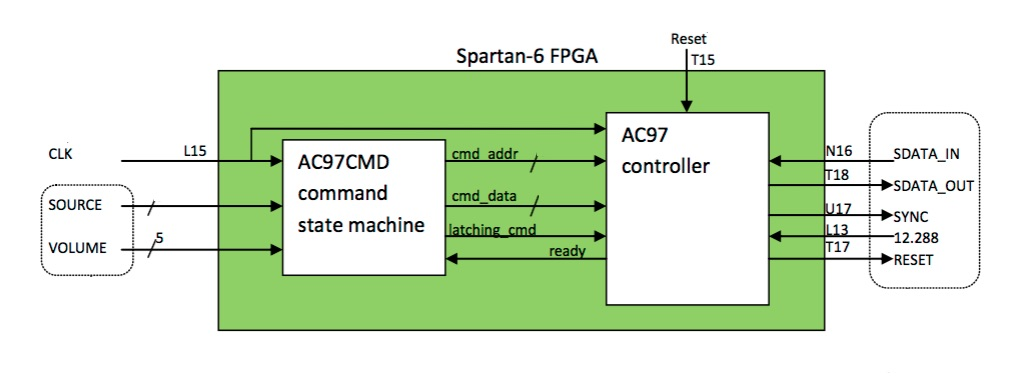
\includegraphics[scale=0.5]{images/snd_gen.jpg}
		\caption{Block diagram of the Sound Generator}
		\label{snd_gen}
	\end{figure}
